\chapter{SVD and Low-Rank Approximation}

\section{Singular Value Decomposition (SVD)}
Let us suppose that there is a matrix $A \in \R^{m \times n}$ whose rank is $rk(A) = r$, then there exists a decomposition of $A$ in the shape of:
\[
    A = \sum_{i = 1}^n \sigma_i \vec{u_i} \vec{v_i}^T
\]
where,
\begin{bindenum}
    \item The set $\{\vec{u_1}, \dots, \vec{u_n}\}$ is orthonormal
    \item The set $\{\vec{v_1}, \dots, \vec{v_n}\}$ is orthonormal
    \item $\forall i \in [1, r], \sigma_i > 0$
    \subitem $\forall i \in [1, n], \sigma_i \geq 0$
\end{bindenum}
\begin{ln-symbol}{Compact SVD}{}
    The above dyadic decomposition of SVD written in terms of matrix transformation would be:
    \begin{align*}
        A &=
        \begin{bmatrix} \vec{u_1} & \cdots & \vec{u_r} \end{bmatrix}
        \begin{bmatrix}
            \sigma_1 & & \\
            & \ddots & \\
            & & \sigma_r
        \end{bmatrix}
        \begin{bmatrix} \vec{v_1}^T \\ \vdots \\ \vec{v_r}^T \end{bmatrix} \\
        &= U_r \Sigma_r V_r^T
    \end{align*}
\end{ln-symbol}
Meanwhile, the full SVD that still considers zero-valued $\sigma_i$ is written as follows:
\begin{ln-symbol}{Full SVD}{}
    The formulation follows:
    \begin{align*}
        A &=
        \begin{bmatrix} \vec{u_1} & \cdots & \vec{u_m} \end{bmatrix}
        \begin{bmatrix}
            \Sigma_r & 0 \\
            0 & 0
        \end{bmatrix}
        \begin{bmatrix} \vec{v_1}^T \\ \vdots \\ \vec{v_n}^T \end{bmatrix} \\
        &= U \Sigma V^T
    \end{align*}
    from which, we may observe that the shape of $\Sigma$ is highly dependent on the shape of $A$:
    \begin{bindenum}
        \item If $A$ is tall, so is $\Sigma$
        \item If $A$ is wide, so is $\Sigma$
    \end{bindenum}
\end{ln-symbol}
The squareness of $U$ and $V$ in full SVD allows us to also decompose $A^T A$ as:
\[
    A^T A = {(U \Sigma V^T)}^T (U \Sigma V^T) = V \Sigma^T U^T U \Sigma V^T = V \Sigma^2 V^T
\]
which is more convenient than the compact form SVD that instead uses rectangular $U$ and $V$.

\subsection{Formation of SVD}
As singular vectors are eigenvectors of symmetric matrices $A^T A$, by applying Spectral Theorem, we find that singular vectors of $A$ would all be orthonormal.
Then, let's use this point as an opportunity to praise $A^T A$'s symmetricness:
\begin{ln-theorem}{The Properties and Formation of SVD}{}
    Let the nonzero eigenvalues of $A^T A$ be
    \[
        \lambda_1 \geq \cdots \geq \lambda_r > 0
    \]
    where, upon dimming that $rk(A^T A) = r$, we may obtain $rk(A) = rk(A^T A) = r$ (using rank-nullity theorem, and the fact that $N(A^T A) = N(A)$). \\
    Let us also suppose that orthonormal vectors in $V$ form eigenpairs with the above eigenvalues:
    \[
        \forall i \in [1, r], A^T A \vec{v_i} = \lambda_i \vec{v_i}
    \]
    Now, define that,
    \[
        \sigma_i := \sqrt{\lambda_i}
    \]
    such that:
    \[
        \vec{u_i} := \frac{A \vec{v_i}}{\sigma_i}
    \]
\end{ln-theorem}
Let us now check, whether the above formation grants an orthonormal $U$:
\begin{ln-explain}{Orthonormality of Set of $\vec{u_i}$}{}
    Let us follow the definition of $\vec{u_i}$ from the last block. \\
    Then,
    \[A \vec{v_i} = \sigma_i \vec{u_i}\]
    Suppose now we have some vectors $\vec{u_i}$ and $\vec{u_j}$, then
    \begin{align*}
        \vec{u_i} \cdot \vec{u_j}
        &= \frac{\vec{v_i}^T A^T}{\sigma_i} \frac{A \vec{v_j}}{\sigma_j} \\
        &= \frac{\vec{v_i}^T \lambda_j \vec{v_j}}{\sigma_i \sigma_j} = 0
    \end{align*}
\end{ln-explain}
Now that we have proven the orthonormality and note the definitions of $\vec{u_i}$ and $\vec{v_i}$, we arrive at the conclusion:
\[
    A V = U \Sigma, A = U \Sigma V^T
\]
such arithmetic operation is only possible under the full SVD form (such that $V$ can be noted as orthonormal at all).
This is once again a demonstration of significance of full SVD.

\subsection{Geometry of SVD}
\begin{ln-fig}{Geometric Property of SVD as Transformation}{}
    We may see from the below image's operations,
    \begin{center}
        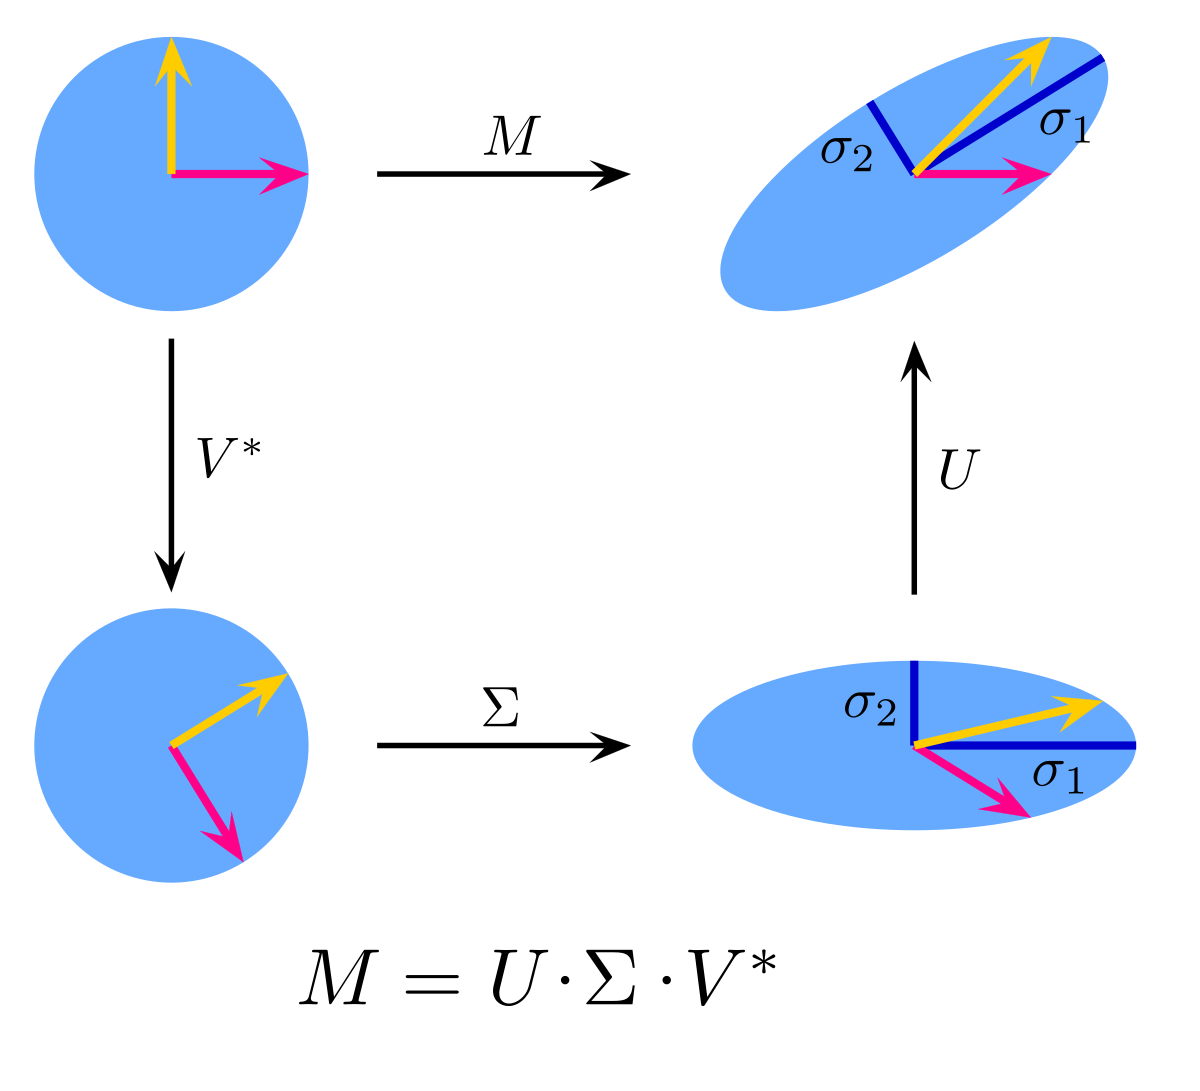
\includegraphics[scale=0.1]{figs/ln05/svd_geometry.png}
    \end{center}
    that SVD is, as priorly mentioned, a combination of three transformations. Where,
    \begin{bindenum}
        \item The orthonormal matrices $U$, $V$ are reflections or rotations.
        \item The matrix $\Sigma$ is a dilation.
    \end{bindenum}
    Furthermore, let us observe the vectors drawn on the unit circle. \\
    Since $V$ is orthonormal, we may conclude that $\vec{v_1} \perp \vec{v_2}$. However, bizzarely, we may also find that
    \[A \vec{v_1} \perp A \vec{v_2}\]
\end{ln-fig}

\section{Low Rank Approximation}
Low Rank Approximation is the task of approximating a matrix $A$ in a lower rank than $rk(A)$, to conserve computational cost and perform efficient computations.

\subsection{Matrix Norms}
Let us first discuss the optimization function of this task: matrix norm.

The norm of matrix also comes in diverse form, because matrices can be interpreted in many forms. \\
For example:
\begin{bindenum}
    \item Chunk of data (like an array)
    \item Operator of transformation
\end{bindenum}
Therefore, along these interpretations, we may present respective definitions of matrix norms.
\begin{ln-define}{Frobenius Norm}{}
    \textit{insert most recent COMPSCI 189 weeder homework PTSD.} \\
    The Frobenius Norm is defined as:
    \[
        \pnorm{A}{F} = \sqrt{\sum_{i = 1}^m \sum_{j = 1}^n A_{i,j}^2} = \sqrt{Trace(A^T A)}
    \]
    This is because the Frobenius inner product may be defined as:
    \[
        {\langle A, B \rangle}_F = Trace(A^T B) = \sum_{i = 1}^n \vec{A_i} \cdot \vec{B_i}
    \]
    and, as we recognize the relation between norm and inner product,
    \[
        \pnorm{A}{F} = \sqrt{{\langle A, A \rangle}_F} = \sqrt{\sum_{i = 1}^n \vec{A_i} \cdot \vec{A_i}}
    \]
\end{ln-define}
The Frobenius Norm has some interesting properties:
\begin{ln-theorem}{Orthonormal Matrices and Frobenius Norm}{}
    Let $U_1 \in \R^{m \times m}$, $A \in \R^{m \times n}$, and $U_2 \in \R^{n \times n}$, where $U_1, U_2$ are orthonormal. \\
    Then,
    \begin{align*}
        \pnorm{U_1 A}{F}
        &= \sqrt{Trace(A^T U_1^T U_1 A)} \\
        &= \sqrt{Trace(A^T A)} = \pnorm{A}{F} \\
        \pnorm{A U_2}{F}
        &= \sqrt{Trace(U_2^T A^T A U_2)} \\
        &\underset{\text{Commutivity in Trace}}{=} \sqrt{Trace(A^T A)} = \pnorm{A}{F} \\
    \end{align*}
\end{ln-theorem}
Now, let's discuss another definition of matrix norm:
\begin{ln-define}{Operator Norm (aka. Spectral Norm, L2-Norm)}{}
    Such norm is defined as:
    \[
        \pnorm{A}{2} = \max_{\pnorm{\vec{x}}{2} = 1} \pnorm{A \vec{x}}{2} = \sigma_{max}(A)
    \]
    \tcblower
    \textbf{Solution to Above Optimization Problem.}
    \begin{align*}
        \max_{\pnorm{\vec{x}}{2} = 1} \pnorm{A \vec{x}}{2}
        = \max_{\pnorm{\vec{x}}{2} = 1} \sqrt{\vec{x}^T A^T A \vec{x}}
        = \sqrt{\lambda_{max}(A^T A)} = \sigma_{max}(A)
    \end{align*}
    Suppose we attach another orthonormal matrix $U$ to the original matrix $A$, then the optimization problem develops a solution fairly similaly:
    \begin{align*}
        \max_{\pnorm{\vec{x}}{2} = 1} \pnorm{AU \vec{x}}{2}
        &= \max_{\pnorm{\vec{x}}{2} = 1} \sqrt{\vec{x}^T U^T A^T A U \vec{x}} \\
        &= \max_{\pnorm{\vec{x}}{2} = 1} \sqrt{\vec{y}^T A^T A \vec{y}} \\
        &= \sqrt{\lambda_{max}(A^T A)} = \sigma_{max}(A)
    \end{align*}
    where since we still find that $\vec{y}$ is normal, the attachment of $U$ providing no change to the optimization problem. \\
    Meanwhile, we find this phenomenon to persist even if $U$ is multiplied from an opposite direction:
    \begin{align*}
        \max_{\pnorm{\vec{x}}{2} = 1} \pnorm{UA \vec{x}}{2}
        &= \max_{\pnorm{\vec{x}}{2} = 1} \sqrt{\vec{x}^T A^T U^T U A \vec{x}} \\
        &= \max_{\pnorm{\vec{x}}{2} = 1} \sqrt{\vec{x}^T A^T A \vec{x}} \\
        &= \sqrt{\lambda_{max}(A^T A)} = \sigma_{max}(A)
    \end{align*}
    Therefore, we may also observe similar properties in norms, where:
    \[
        \pnorm{A}{2} = \pnorm{U_1A}{2} = \pnorm{AU_2}{2} \text{ for orthonormal matrices } U_1, U_2
    \]
\end{ln-define}

